%!TEX root = ../main.tex

\newcommand{\fnaRetrievalTime}{\formatdate{25}{11}{2014} at \formattime{9}{14}{0}}

\chapter{Ribofinder}
\label{ch:rfinder}

\lhead{Ribofinder: A \Rb Detection Pipeline}

\section{Introduction}
\label{sec:rfinder:intro}

In this chapter, we present the \rfinder program---a pipeline to facilitate the
detection of putative \grbs across genomic data. The \rfinder
tool operates in three stages. First we use \infernal \cite{infernal} and \tthp \cite{ermolaeva:2000cl} to detect
putative aptamers and expression platforms, two distinct components of
\rbs described in section \ref{sec:rfinder:bkgrnd}. After coalescing
this data into a pool of candidate \rbs, we use \rfold \cite{lorenz.amb11} with constraints
based on experimental data to compute the two distinct structural
conformations---`gene on' and `gene off'. In the third and final stage, we
leverage \foldalign \cite{havgaard:2007ca} to measure the similarity between our candidate pool and a
canonical \grb well studied in the literature, the
xanthine phosphoribosyltransferase (xpt) \grb from {\em Bacillus subtilis}. At the time
of this writing, Prof. Dr. Mario
M\"orl at Universit\"at Leipzig is overseeing preliminary structural
validation of predicted gene on and off structures for a number of
computationally predicted \grbs in {\em B. megaterium}.

\subsection{Organization}
\label{subsec:rfinder:org}

This chapter is organized in the following fashion. After providing background
on the structural components of a \rb alongside their biological
significance, we outline the deficiencies in the `state of the art' software
when as it relates specifically to \rb detection. We then move on to outline
the three stages of \rfinder: candidate selection, structural prediction, and
candidate curation. Having described the approach of the software, we move on
to present our findings in using \rfinder to detect \grbs across
the bacterial RefSeq database. Finally, we provide brief commentary on possible
extensions of the algorithm to locate other flavors of \rbs, of which
adenine-sensitive aptamers are a straightforward extension.

\section{Background}
\label{sec:rfinder:bkgrnd}

Riboswitches are regulatory mRNA elements that modulate gene expression via
structural changes induced by the direct sensing of a small-molecule metabolite.
Most often found in bacteria, riboswitches regulate diverse pathways including the
metabolism and transport of purines, methionine, and thiamin amongst others. The
structure of a riboswitch includes an aptamer domain---involved in the direct
sensing of the small-molecule---and a downstream expression platform whose
structure changes upon the aptamer binding the metabolite. Because of the
discriminatory nature of metabolite sensing, groups have had great success in
finding representative examples of aptamers across a diverse collection of
bacterial species; RFam 12.0 currently contains 26 different families of aptamers
involved in different metabolic pathways. Whereas there exists strong sequence and
structural similarity within the aptamer of a riboswitch family, the expression
platform is highly variable, and thus challenging to capture using traditional
SCFG-based approaches. For this reason databases such as RFam only contain the aptamer
portion of the riboswitch, and there exists no database providing sequences
including expression platforms, necessary for capturing the `on' and `off'
conformations of this regulatory element. We have developed a new pipeline---
called \rfinder---which can detect putative riboswitches including their
expression platforms and likely conformational structures across a wide collection
of genomic sequences.

\section{The \rfinder pipeline}
\label{sec:rfinder:pipeline}

At the time of our retrieval (\fnaRetrievalTime), the RefSeq database hosted by
NCBI comprised 5,121 complete bacterial genomes with corresponding genomic
annotations. In order to both detect putative full riboswitches across this
collection of data as well as filter the candidates down to a number tractable for
experimental validation, we developed a novel pipeline which takes a three-tiered
approach to candidate selection. Our approach is to
\begin{inparaenum}[\em 1\upshape)]
\item identify a pool of candidate riboswitches across genomic data;
\item perform a coarse-grained filtering of the candidate pool based on structural
characteristics; and finally
\item fine-grained curation of the candidates based on a collection of measures
and pairwise similarity.
\end{inparaenum} Figure \ref{fig:rfinder:flowchart} outlines this approach as a
flowchart.

\begin{figure}[!ht]
\centering
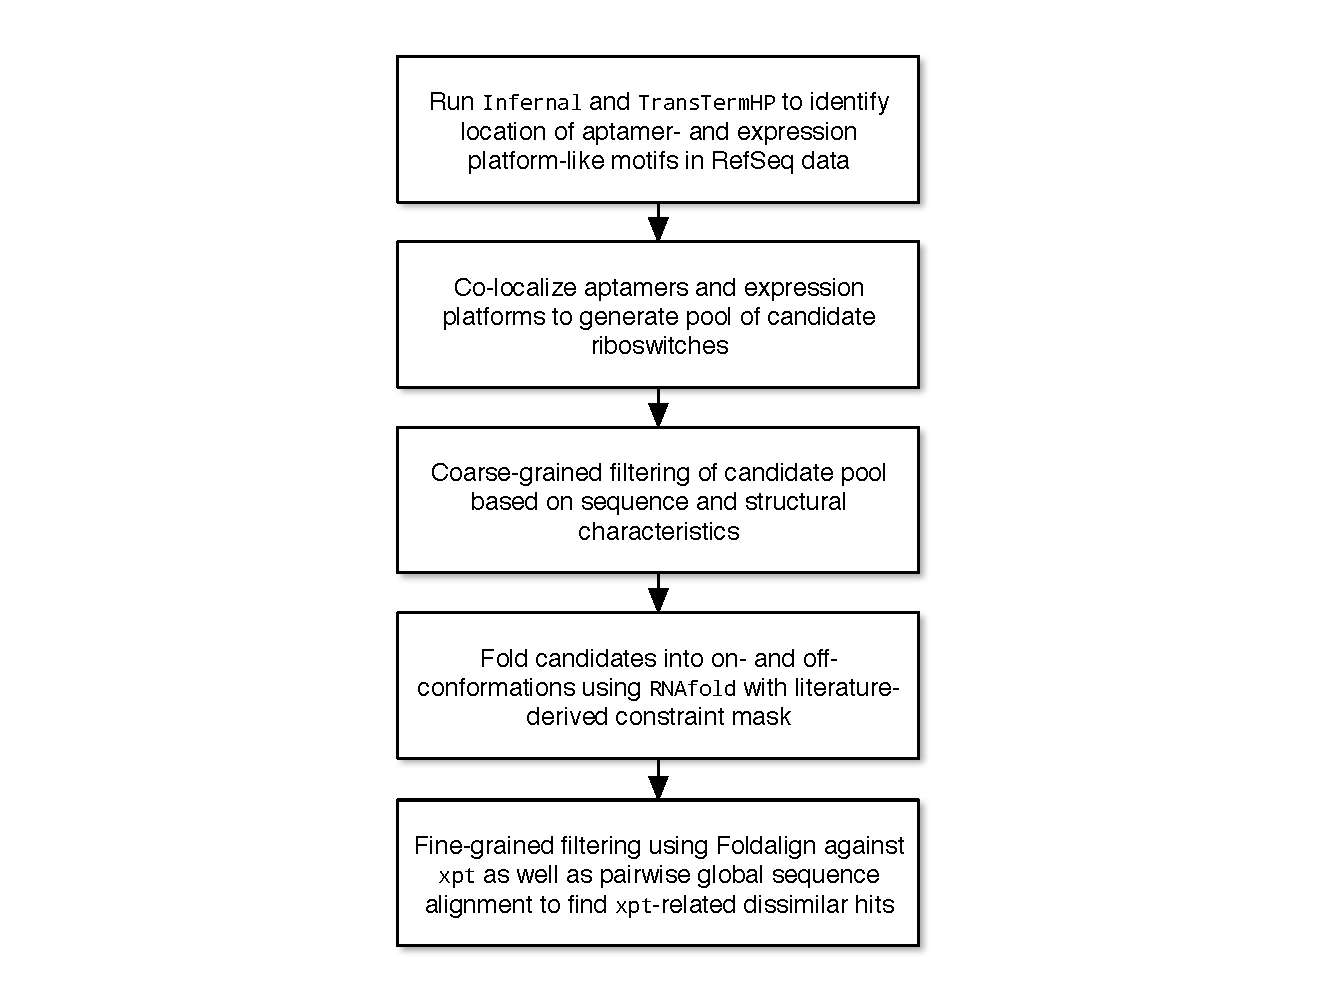
\includegraphics[width=.9\textwidth]{Figures/Ribofinder/ribofinderOverview.pdf}
\caption{Outline of the approach for the \rfinder pipeline.}
\label{fig:rfinder:flowchart}
\end{figure}

In the following discussion, we describe the application of \rfinder to identify unannotated guanine purine riboswitches; guanine-sensing cis-regulatory elements which modulate the expression of genes involved in purine biosynthesis.

\subsection{Step 1: Candidate selection}
\label{subsec:rfinder:selection}

The RefSeq data we used for analysis contains 5,121 annotated bacterial genomes across 2,732 different organisms, totaling over $9.5 * 10^9$ bases. We used the program \infernal to determine the coordinates of putative aptamer structures within the RefSeq genomes, and \tthp to locate candidate rho-independent transcription terminators.

\subsubsection{Detecting Aptamers with \infernal}
\label{subsubsec:rfinder:infernal}

\infernal \cite{infernal} uses a stochastic context-free grammar (SCFG) with a user-provided multiple sequence alignment (MSA) to efficiently scan genomic data for RNA homologs, taking into consideration both sequence and structural conservation. Using the purine aptamer MSA from RFam 12.0 (RF00167), \infernal (v1.1.1, default options) detects 1,537 significant hits having E-value $<= 0.01$. Because \infernal leverages the concept of a `local end'---a large insertion or deletion in the alignment at reduced cost---it is possible for the software to return a significant hit whose aligned structure does not have the canonical three-way junction observed in all purine riboswitches. \rfinder prunes these truncated \infernal hits by converting the alignment structure into a parse tree, and only permitting trees of sufficient complexity to contain a multiloop (described further in \ref{subsubsec:rfinder:shapes}). The pyrimidine residue abutted next to the P1 stem in the J3--1 junction differentiates between guanine and adenine-sensing riboswitches by binding the complimentary purine ligand; for our interest in \grbs exclusively we require the presence of a cytosine at this residue. In total, using \infernal with these additional filters yields 1,280 guanine aptamers across 555 unique organisms (note: here and elsewhere I define a `unique organism' as having a unique taxonomy ID).

\subsubsection{Detecting Expression Platforms with \tthp}
\label{subsubsec:rfinder:tthp}

\tthp \cite{ermolaeva:2000cl} detects rho-independent terminators in bacterial genomes in a context-sensitive fashion by leveraging the protein annotations available in PTT data. These terminator sequences canonically have a stable hairpin loop structure immediately preceding a run of $5+$ uracil residues, the combination of which causes the ribosomal machinery to stall and dissociate from the transcript. \tthp performs a genomic scan to determine candidate loci with this motif, and returns scored hits. The scoring system considers both structural homology and the genomic contextual information available in the PTT file. Across our collection of bacterial genomes acquired from NCBI RefSeq data, \tthp identified 2,752,469 rho-independent terminators using the default filters.

Due to the spatially-mediated structural regulation of purine riboswitches, whereby ligand interaction with the aptamer domain induces local structural rearrangement in the expression platform, we paired aptamers with corresponding terminators by minimizing the genomic distance, with an upper bound of 200 nucleotides between the end of the aptamer domain and start of the terminator. This approach yields 577 candidate riboswitches, 81 of which have multiple rho-independent terminators within range of a putative aptamer produced by \infernal. For these, we simply pair the closest \tthp hit with the aptamer domain.

\begin{figure}[!ht]
\centering
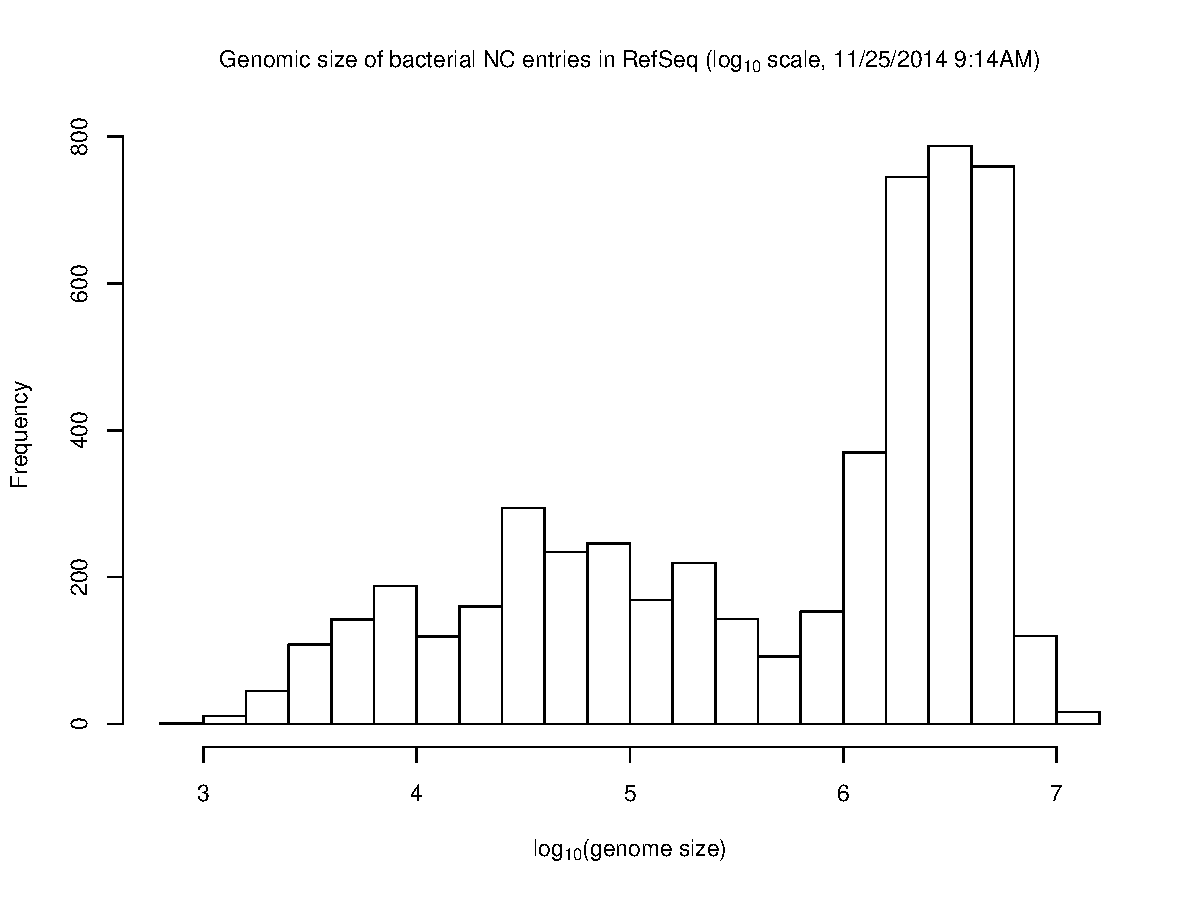
\includegraphics[width=.9\textwidth]{Figures/Ribofinder/refseqGenomeSizes.pdf}
\caption{Histogram displaying the distribution of genome sizes across the RefSeq
data analyzed, comprising 5,172 bacterial genomes. Genome size is shown using a
$\log_{10}$ scale.}
\label{fig:genomeSizes}
\end{figure}

\subsection{Step 2: Structural prediction}
\label{subsec:rfinder:strpred}

Until this point we have been focused on the generation of candidate sequences
from our RefSeq dataset, without yet focusing on the specifics of underlying
secondary structures for these candidates. In the following section, we explain
how constraint folding is used to generate putative `on' and `off' conformations
for each candidate.

\subsubsection{Notation for Representing Abstract RNA Shapes}
\label{subsubsec:rfinder:shapes}

Given an RNA sequence $\seq = \seqN$, where positions $s_i$ are drawn from the collection of single-letter nucleotide codes, i.e.
$s_i \in \{\text{A,\,U,\,G,\,C}\}$, it is possible to describe a corresponding
secondary structure \strS compatible with \seq using the dot-bracket notation.
In this notation, each nucleotide $a_i$ has a corresponding state $s_i$, where
$s_i$ is denoted as a `.' if unpaired and a `(' [resp. `)'] if the left [resp.
right] base in a base pair. Given any two base pairs $(i,j)$ and $(k,l)$ in \strS, then $i < k < j \iff i < l < j$; pseudoknots are not permitted in the structure. A secondary structure taking this form is said to have balanced parentheses, and can additionally be represented using a context-free grammar such as:

\begin{equation} \label{eq:str_cfg}
S \rightarrow S\,.\;|\;.\,S\;|\;(S)\;|\;SS\;|\;\epsilon
\end{equation}

The grammar from \eqref{eq:str_cfg} can be used to generate a parse tree \tree for \strS. The benefit of working with \tree over \strS is that the parse tree offers an abstract representation of secondary structure shape independent of sequence length, permitting us to classify and eventually constrain a large collection of sequences having variable length which are all expected to have the same abstract tree shape. This is analogous to what the Giegerich lab refers to as their `type 5' structural abstraction using the \rshapes tool. Every node in \tree represents a helix in \strS, and internally tracks the indices of both its beginning $(i,j)$ and closing $(k,l)$ base pair. We use a level-order naming convention to refer to helices within the parse tree, whereby a position \treePos{p}{1} references the first child of the root node, \treePos{p}{1,2} references the second child of \textdown{\ms{p}}{1}, and generally \treePos{p}{$i_1,i_2,\cdots,i_n$} refers to the $i_n$\textsuperscript{th} child of \treePos{p}{$i_1,i_2,\cdots,i_{n-1}$}. To reference specific nucleotides in the context of their location relative to a helix, we use the opening and closing base pairs $(i,j)$ and $(k,l)$ as landmarks. Thus, \treeIdx{p}{1}{l} is the index in \strS of the right-hand side closing base pair of \treePos{p}{1}. We use the notation \treePos{t}{$i$} to refer to the subtree of \tree whose root is \treePos{p}{$i$}.

Finally, we introduce the concept of a tree signature. The tree signature for a tree \tree is a list of the node depths when traversed in a depth-first pre-order fashion. To provide a concrete example, consider the following experimentally validated xpt \grb from Bacillus subtilis subsp. subtilis str. 168 (NC\_000964.3 2320197--2320054) with corresponding gene off structure as seen in Figure \ref{fig:rfinder:xptOff}.
\medskip

\begin{figure}[!ht]
\centering
\begin{subfigure}[h]{\textwidth}
\centering
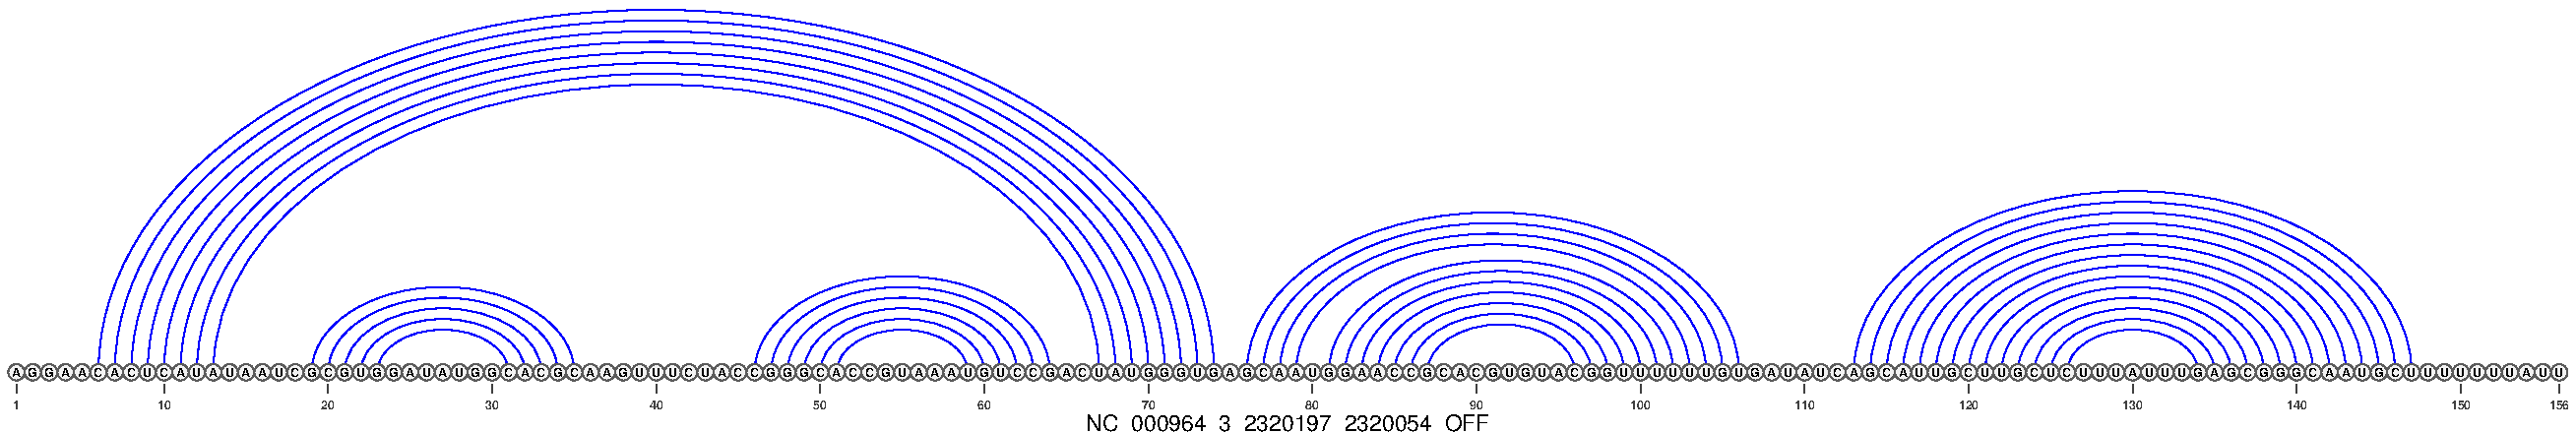
\includegraphics[width=.9\textwidth]{Figures/Ribofinder/NC_000964_3_2320197_2320054_OFF.pdf}
\end{subfigure} \\
\medskip
\begin{subfigure}[h]{\textwidth}
\centering
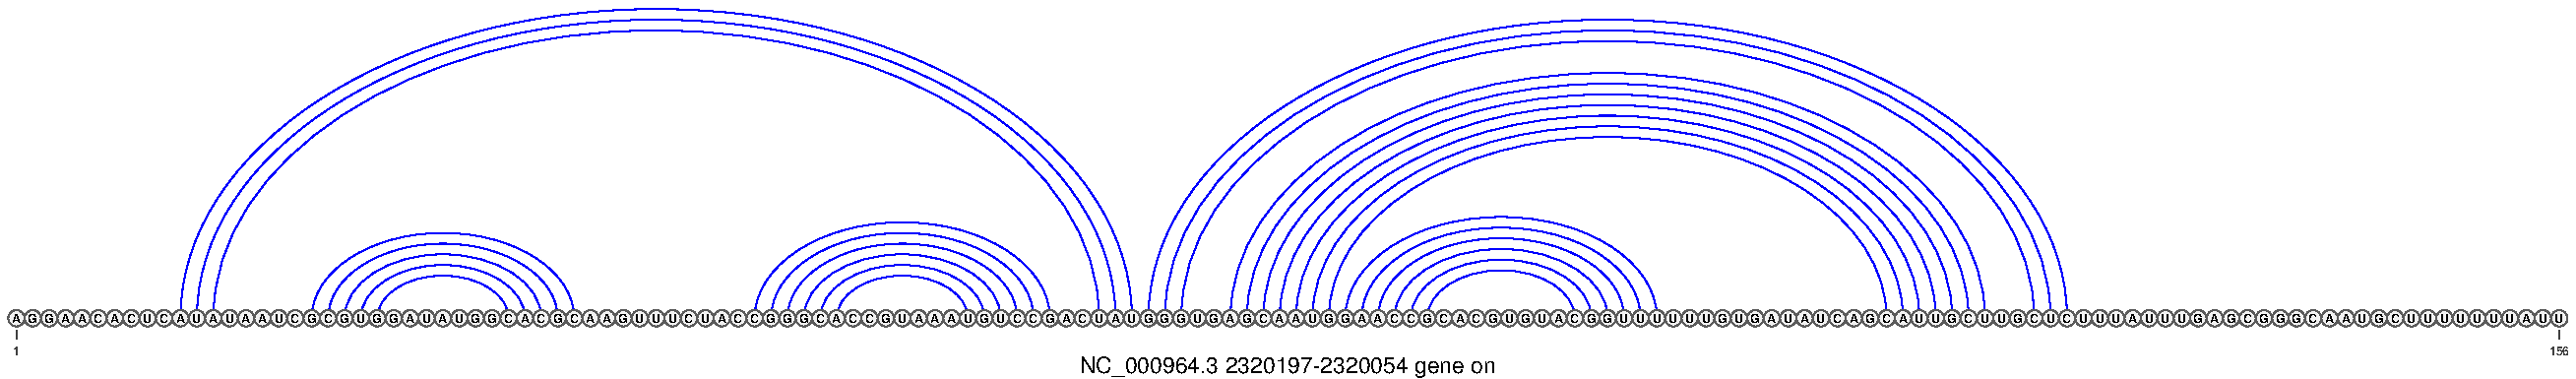
\includegraphics[width=.9\textwidth]{Figures/Ribofinder/NC_000964_3_2320197_2320054_ON.pdf}
\end{subfigure}
\caption{{\em (Top)} The xanthine phosphoribosyltransferase (xpt) \grb from
{\em B. subtilis} subsp. subtilis str. 168 (NC\_000964.3 2320197--2320054),
and corresponding gene off structure derived from crystallography analysis in
complex with guanine \cite{breaker:riboswitch2}. {\em (Bottom)} The experimentally
derived gene on structure for \Bsxpt.}
\label{fig:rfinder:xptOff}
\end{figure}

The \rshapes `type 5' representation for this structure is \ms{[[][]][][]} (note the coalesced left bulge in the hairpin immediately downstream the closing multiloop stem, at helix \treePos{p}{2}) and the tree signature for this parse tree of the structure is \ms{[0,1,2,2,1,1]}.

We leverage the notion of abstract structural filtering initially to ensure that all \infernal aptamer hits have a tree signature of \ms{[0,1,2,2]}, which represents a three-way junction, and that the binding site for the guanine ligand $\treeIdx{p}{1}{l - 1} = \text{C}$. These filters, in combination with the proximal terminator hairpins produced by \tthp yield the aforementioned 577 candidate \grbs for which we then try to produce reasonable gene on and off structures.

\subsubsection{Constrained Folding to Predict Switch Structures}
\label{subsubsec:rfinder:consfold}

To restrict our search to unannotated \grbs, and further ensure that we are not re-detecting sequences based off the RFam covariance model provided to \infernal, we constrain our search to those RefSeq organisms not represented in the RFam seed alignment. 503 of the 577 candidates, or 87.18\% represent putative unannotated riboswitches not represented by RF00167.

The gene off structure \strOff for a \grb is the easier of the two to find computationally, since the terminator loop is exceptionally thermodynamically stable. In the gene on conformation \strOn, the P1 stem of the multiloop partially dissociates and an anti-terminator loop forms between the region immediately 3' of the P1 stem and what was the left-hand side of the terminator loop. This truncated P1 stem, which closes the three-way junction in the aptamer, is exceptionally unstable based on present energy models available for structural folding, and requires special treatment to reconstitute in our final structures.

The software \rfold (v2.1.8) allows for the folding of RNA molecules with `loose' constraints. In this model of constrained folding, the resulting structure produced by the software guarantees not to explicitly invalidate any user-provided constraints, but does not guarantee all constraints will be satisfied in the resulting structure. For each of the candidate \grbs, having \treeFor{\infernal} and \treeFor{\tthp}, we build the following constraint masks:

\begin{center}
\begin{tabularx}{\linewidth}{*{2}{L}}
  \toprule
  Guanine gene off constraint mask & Guanine gene on constraint mask \\
  \cmidrule(lr){1-2}
  \multicolumn{2}{l}{Prohibit base pairing upstream of \treeIdx{p}{1}{i} and
  downstream of \treeIdx{p}{2}{l}.} \\
  \multicolumn{2}{l}{Force base pairs and unpaired regions in \treePos{t}{1}, with
  the exception of \treePos{p}{1}.} \\
  \multicolumn{2}{l}{Prohibit formation of \treePos{p}{1} stem, which closes the
  three-way junction.} \\
  \cmidrule(lr){1-2}
  Force base pairs and unpaired regions in \treePos{t}{2}. &
  Require $m$ nucleotides starting from \treeIdx{p}{1}{l + 3} to pair to the
  right, where $m = len(\treePos{p}{2})$, and require the left-hand side of the
  \treePos{p}{2} helix to pair to the left. \\
  & Disallow pairing downstream of \treeIdx{p}{2}{j}. \\
  \bottomrule
\end{tabularx}
\end{center}

These constraint masks are run using the command-line flags \ms{-d 0 -P rna\_turner1999.par} to disable dangles and use the Turner 1999 energies respectively. Experimental evidence using inline probing suggests that the `on' conformation of the \grb has a reduced P1 stem length of 3 base pairs; in practice we were unable to force \rfold to respect this constraint regardless of command-line options specified. For this reason we reconstitute the P1 stem in both structures after constrained folding, having length equivalent to it the \infernal P1 stem (resp. 3 base pairs) in the gene off (resp. gene on) structure.

This difficulty with \rfold can be shown by using the constraint-produced structures as exhaustive constraints themselves. All unpaired nucleotides in \strOff and \strOn are notated by a `\ms{x}' and all base pairs by `\ms{()}' for the 5' and 3' side of the pair respectively to form new constraints mask \strConst{off} and \strConst{on}, having all bases' state explicitly specified. By refolding all 577 candidate sequences with \strConst{off} and \strConst{on} using the same options as before, only 463 (or 80.24\%) of the resulting structures from \strConst{off} have the tree signature prefix \ms{[0,1,2,2,1]}, and just 21 (or 3.64\%) of the \strConst{on} structures correctly re-fold their multiloop.

\begin{figure}[!ht]
\centering
\begin{subfigure}[h]{\textwidth}
\centering
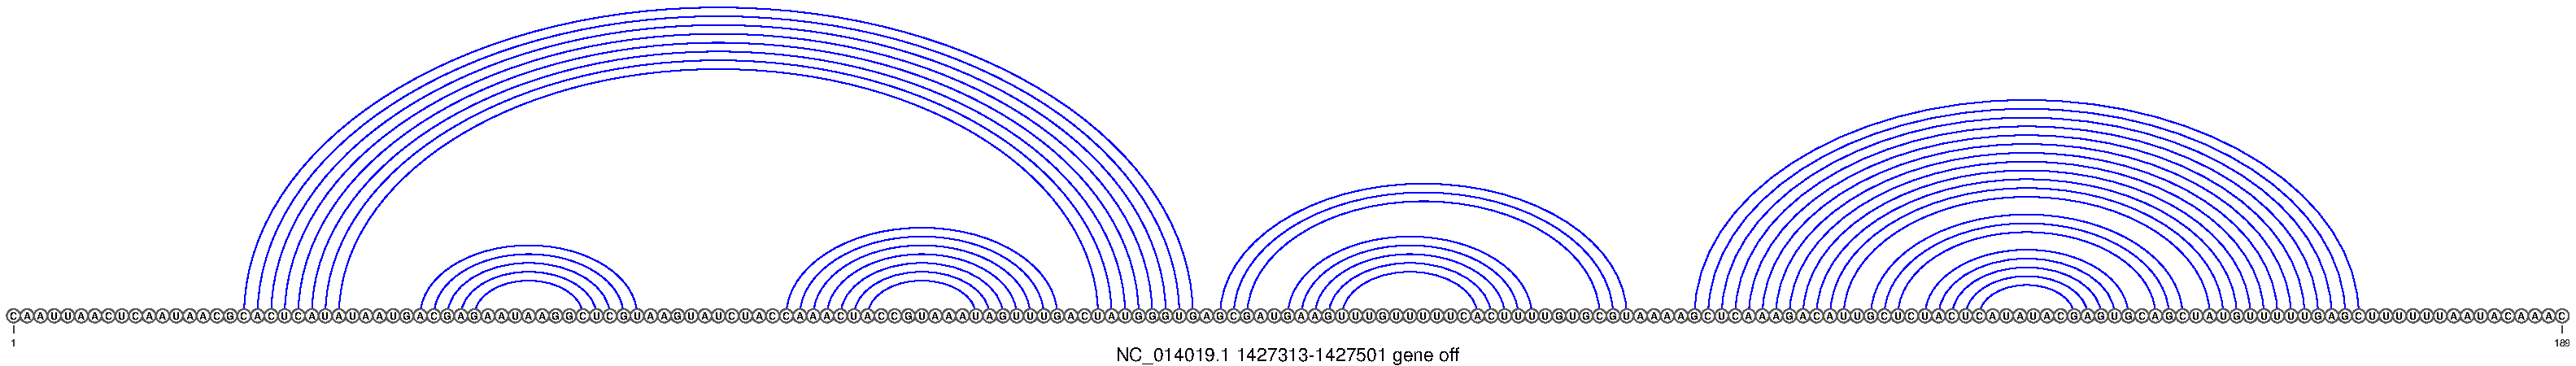
\includegraphics[width=.9\textwidth]{Figures/Ribofinder/NC_014019_1_1427313_1427501_OFF.pdf}
\end{subfigure} \\
\medskip
\begin{subfigure}[h]{\textwidth}
\centering
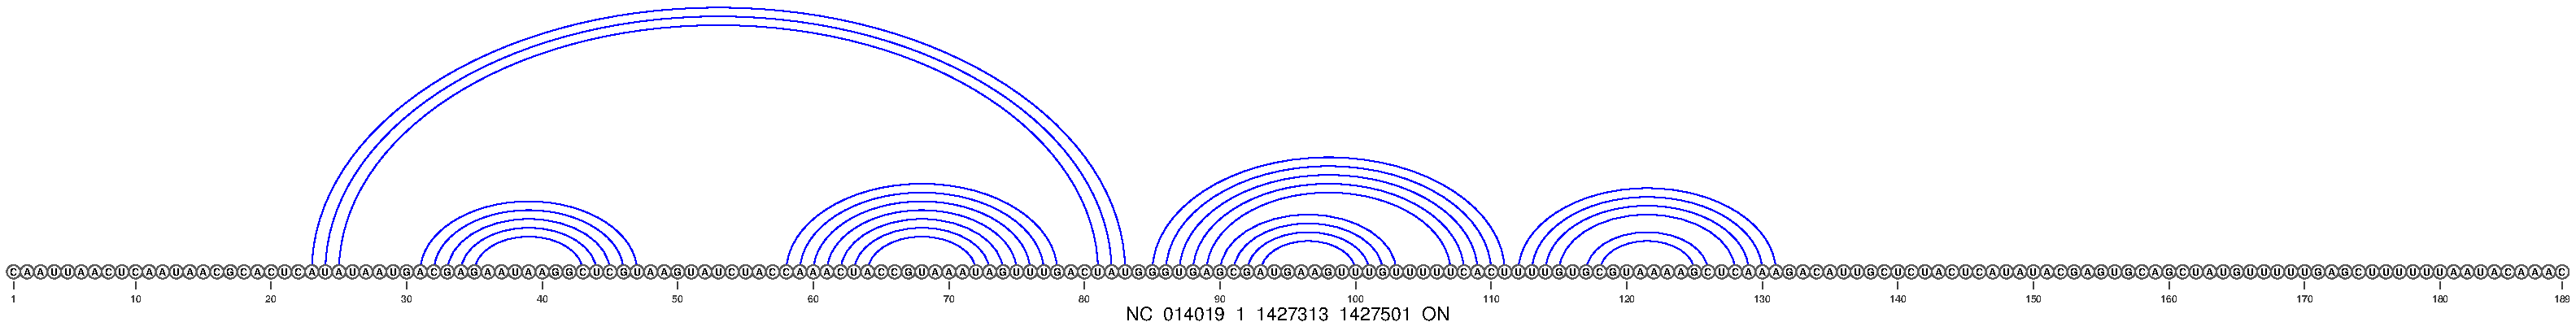
\includegraphics[width=.9\textwidth]{Figures/Ribofinder/NC_014019_1_1427313_1427501_ON.pdf}
\end{subfigure}
\caption{{\em Top:} the computationally predicted gene off conformation of sequence NC\_014019.1 1427313--1427501, using \rfold from the ViennaRNA 2.1.8 suite, with dangles disabled and the Turner 1999 energies. This sequence is located upstream of the xpt gene in {\em B. megaterium} QM B1551. {\em Bottom:} the gene on conformation.}
\label{fig:example_ss}
\end{figure}

\subsection{Step 3: Candidate curation}
\label{subsec:rfinder:curation}

Until now, we have described our approach for generating the 503 \grb candidates
in RefSeq, alongside their gene on and off structures. Unfortunately the
experimental validation of all 503 candidates is not tractable, so it was
necessary to reduce this collection again to a more manageable size, while only
keeping the most promising candidates. Our original approach involved using
\foldalign alongside the \ms{needleall} tool from XXX \cite{xxx}, to simultaneously
select sequences which closely approximate the more thermodynamically stable
gene off conformation of the experimentally known \Bsxpt \grb, while minimizing
sequence similarity between candidates selected for experimental validation. Due to
experimental constraints, we elected finally to instead choose a small number
($n = 2$) of organisms easily available which had multiple promising hits as our
experimental candidate pool.

\section{Using \rfinder against the RefSeq database}
\label{sec:rfinder:refseq}

\section{Extending beyond \grbs}
\label{sec:rfinder:ext}
